\documentclass[embeddedlogo]{ufsc-thesis-rn46-2019}

\usepackage[T1]{fontenc} % fontes
\usepackage[utf8]{inputenc} % UTF-8
\usepackage{lipsum} % Gerador de texto
\usepackage{pdfpages} % Inclui PDF externo (ficha catalográfica)
\usepackage{biblatex} %Imports biblatex package

% Usado para mostrar código
\usepackage{minted}
\newmintinline[mt]{latex}{fontsize=\normalsize}
\newmintinline[mft]{latex}{fontsize=\footnotesize}
\setminted{fontsize=\tiny,linenos,xleftmargin=2em}
\setmintedinline{breaklines,breakbytokenanywhere}

% Usado para mostrar comandos latex nesse guia:
\newcommand{\lacmd}[1]{\texttt{\textbackslash{}#1}}
\newcommand{\laenv}[1]{\texttt{\textbackslash{}begin\{#1\}...\textbackslash{}end\{#1\}}}
\newcommand{\laenvi}[2]{\texttt{\textbackslash{}begin\{#1\}[#2]...\textbackslash{}end\{#1\}}}

%%%%%%%%%%%%%%%%%%%%%%%%%%%%%%%%%%%%%%%%%%%%%%%%%%%%%%%%%%%%%%%%%%%%
%%% Configurações da classe (dados do trabalho)                  %%%
%%%%%%%%%%%%%%%%%%%%%%%%%%%%%%%%%%%%%%%%%%%%%%%%%%%%%%%%%%%%%%%%%%%%

% Informações para capa e folha de rosto/certificacao

% Caso o título contenha alguma porção LaTeX ilegível, defina um título
% alternativo opcional com []'s para ser usado no campo Title do PDF
% IMPORTANTE: Os títulos deveriam ser iguais. Apenas use um título
% alternativo se o título não puder ser expresso com letras e números
\titulo[Template \LaTeX{} com metadados]%
       {Desenvolvimento de um Ambiente para Aprendizado e Prática de Técnicas de Segurança Ofensiva em Aplicações Web Vulneráveis}

\autor{Samuel Cardoso}
\data{2022} % ou \today
\instituicao{Universidade Federal de Santa Catarina}
\centro{Centro Tecnológico}
\local{Florianópolis} % Apenas cidade! Sem estado
%\programa{Programa de Pós-Graduação em Ciência da Computação}
% Os dois próximos itens são usados para gerar o \preambulo
\tcc % ou \dissertacao ou \tcc
%\titulode{doutor em Ciência da Computação}

%%% Atenção! No caso de TCC, além de usar \tcc, outros comandos devem ser fornecidos:
%%%
% \tcc
\departamento{Departamento de Informática e Estatística}
\curso{Ciências da Computação}
\titulode{Bacharel em Ciência da Computação}
% %% Para TCCs, orientadores e coorientadores podem ser externos, logo a
% %% BU exige que sua afiliação seja explicitada. Por padrão, assume-se
% %% UFSC. Você pode alterar a afiliação com os comandos abaixo:
% \afiliacaoorientador{Universidade Federal de Santa Catarina}
% \afiliacaocoorientador{Universidade Federal da Terra de Ninguém}

% Orientador, coorientador, membros da banca e coordenador
% As regras da BU agora exigem que Dr. apareça **depois** do nome
% Dica: para gerar Profᵃ. use Prof\textsuperscript{a}.
% Dica 2: para feminino use \orientadora e \coorientadora
\orientadora{Prof. Carla Merkle Westphall, Dra.}
%\coorientador{}
\membrobanca{Fabricio Bortoluzzi}{Universidade Federal de Santa Catarina}
\membrobanca{Rômulo Augusto Oliveira Cruz Bittencourt de Almeida}{Universidade Federal de Santa Catarina}
%\membrobanca{Prof. Huifen Chan, Dr.}{Universidade Federal da Terra de Ninguém}
% Dica: se feminino, \coordenadora
\coordenador{Prof. Jean Everson Martina, Dr}

\addbibresource{references.bib} %Import the bibliography file

\begin{document}

%%%%%%%%%%%%%%%%%%%%%%%%%%%%%%%%%%%%%%%%%%%%%%%%%%%%%%%%%%%%%%%%%%%%
%%% Principais elementos pré-textuais                            %%%
%%%%%%%%%%%%%%%%%%%%%%%%%%%%%%%%%%%%%%%%%%%%%%%%%%%%%%%%%%%%%%%%%%%%

% Inicia parte pré-textual do documento capa, folha de rosto, folha de
% aprovação, aprovação, resumo, lista de tabelas, lista de figuras, etc.
\pretextual%
\imprimircapa%
\imprimirfolhaderosto*
% Atenção! \cleardoublepages são inseridos automaticamente
% Atenção! esse \protect é importante
%\protect\incluirfichacatalografica{ficha.pdf} ADICIONAR FICHA TECNICA - EU NÃO VOU LEMBRAR DE ADICIONAR ISSO AQUI E O JOSÉ IRÁ ME LEMBRAR DISSO. EU SOU TEIMOSO E DECIDI DEIXAR ESSE COMENTÁRIO MESMO ASSIM
\imprimirfolhadecertificacao

% Listas de "coisas". O * no final faz com que as listas não sejam 
% incluídas como entratas do sumário (\tableofcontents)

% \listoftables*
% \listofalgorithms*
% \listoffigures*
% \tableofcontents*

%\begin{dedicatoria}
  Este trabalho é dedicado à .....
\end{dedicatoria}
%\begin{agradecimentos}
  
\end{agradecimentos}
%\begin{epigrafe}
  For a number of years I have been familiar with the observation that the quality of programmers is a decreasing function of the density of go to statements in the programs they produce \\
  \cite{dijkstra1968}
\end{epigrafe}
\begin{resumo}[Resumo]
  Em um momento onde a tecnologia evolui tão rapidamente, novas vulnerabilidades em aplicações web são encontradas todos os meses enquanto outras são remediadas, isso faz com que o estado da arte da segurança computacional seja atualizado constantemente. Neste contexto, este trabalho se propõe a desenvolver um ambiente para aprendizado e prática de técnicas de segurança ofensiva em aplicações web com vulnerabilidades de alto risco nos últimos anos.

  \vspace{\baselineskip} 
  \textbf{Palavras-chave:} Segurança Ofensiva. Aplicações Web. Vulnerabilidades.
\end{resumo}
%\begin{resumo}[Resumo Estendido]
  \section*{Introdução} 
  A hifenização é alterada para \texttt{brazil}, mesmo para documentos em inglês. Descrever brevemente esses itens exigidos pela BU. Como a RN 95/CUn/2017 é mais recente e impõe outras regras a revelia de regimentos e regulamentos, é mais sábio obedecê-la. Lembre que esse resumo estendido deve term entre 2 e 5 páginas.
  
  \lipsum[1]
  \section*{Objetivos} 
  \lipsum[2]
  \section*{Metodologia} 
  \lipsum[3]
  \section*{Resultados e Discussão} 
  \lipsum[4]
  \section*{Considerações Finais} 
  \lipsum[5]

  \vspace{\baselineskip}  % Atenção! manter igual ao resumo
  \textbf{Palavras-chave:} Palavra-chave. Outra Palavra-chave composta. Bla.
\end{resumo}
\begin{abstract}
  At a time when technology evolves so quickly, new vulnerabilities in web applications are found every month while others are remedied, this means that the state of the art of computer security is constantly updated. In this context, this work proposes to develop an environment for learning and practicing offensive security techniques in web applications with high-risk vulnerabilities in recent years.

  \vspace{\baselineskip} 
  \textbf{Keywords:} Offensive Security. Web Applications. Vulnerabilities.
\end{abstract}

\listoffigures*  % O * evita que apareça no sumário
% \newpage
% \section*{List of Acronyms}
\begin{acronym}
 \acro{USA}{United States of America}
\end{acronym}

\newpage*

%%!TEX root = ../main.tex

\begin{listadesimbolos}

  $\gets$   & Atribuição \\
  $\exists$   & Quantificação existencial \\
  $\rightarrow$   & Implicação \\
  $\wedge$   & E lógico \\
  $\vee$   & Ou lógico \\
  $\neg$   & Negação lógica \\
  $\mapsto$   & Mapeia para \\
  $\sqsubseteq$   & Subclasse (em ontologias) \\
  $\subseteq$   & Subconjunto: $\forall x\;.\; x \in A \rightarrow x \in B$ \\
  $\langle\ldots\rangle$ & Tupla \\
  $\forall$   & Quantificação universal \\
  mmmmm & Nenhum sentido, apenas estou aqui para demonstrar a largura máxima dessas colunas. Ao abrir o ambiente \texttt{listadesimbolos}, pode-se fornecer um argumento opcional indicando a largura da coluna da esquerda (o default é de 5em): \texttt{\textbackslash{}begin\{listadesimbolos\}[2cm] .... \textbackslash{}end\{listadesimbolos\}} \\
  $\alpha$   & Alpha \\
  $\beta$   & Beta \\
  $\gamma$   & Gamma \\
  $\delta$   & Delta \\
  $\epsilon$   & Epsilon \\
  $\zeta$   & Zeta \\
  $\eta$   & Eta \\
  $\theta$   & Theta \\
  $\iota$   & Iota \\
  $\kappa$   & Kappa \\
  $\lambda$   & Lambda \\
  $\mu$   & Mu \\
  $\nu$   & Nu \\
  $\xi$   & Xi \\
  $\pi$   & Pi \\
  $\rho$   & Rho \\
  $\sigma$   & Sigma \\
  $\tau$   & Tau \\
  $\upsilon$   & Upsilon \\
  $\phi$   & Phi \\
  $\bowtie$  & Apertem os cintos, uma quebra de página se aproxima! \\
  $\oslash$   & Não use exclamações em lista de símbolos! \\
  $\varphi$   & Varphi \\
  $\chi$   & Chi \\
  $\psi$   & Psi \\
  $\omega$   & Omega \\

\end{listadesimbolos}


\tableofcontents*%

%%%%%%%%%%%%%%%%%%%%%%%%%%%%%%%%%%%%%%%%%%%%%%%%%%%%%%%%%%%%%%%%%%%%
%%% Corpo do texto                                               %%%
%%%%%%%%%%%%%%%%%%%%%%%%%%%%%%%%%%%%%%%%%%%%%%%%%%%%%%%%%%%%%%%%%%%%
\textual%
    
\chapter{Introdução}

\label{sec.intro}

\section{Motivação}

A democratização da Internet aumentou exponencialmente o uso de Internet no último século, afetando a vida cotidiana e corporativa das pessoas ~\cite{carneiro2022}, porém o aumento do uso da Internet contém consequências. Nos últimos anos problemas com ataques cibernéticos passaram a ser cada vez mais comuns ao redor do mundo e inclusive no Brasil  ~\cite{avila2013brasil}. Em contra ponto, políticas e leis tornam-se mais rigorosas quanto ao tratamento e a proteção de dados ~\cite{Neves_Lopes_Pavani_Sales_2021}, levando a segurança da informação e a segurança computacional a um novo nível de importância.

Para prevenção contra infortúnios, muitas empresas estão utilizando técnicas de segurança ofensiva para monitorar o nível de segurança e aperfeiçoar suas defesas, já que é mais fácil corrigir uma vulnerabilidade ao ter o conhecimento dela ~\cite{vieira2018}. Existem, porém, complicações e barreiras no aprendizado de segurança ofensiva, uma vez que há uma linha tênue entre legalidade e ilegalidade quando se realiza testes em sites de terceiros.

Visto a lacuna existente na área para aplicar o conhecimento teórico acerca de segurança ofensiva de forma prática, este trabalho se propõe a desenvolver um ambiente para aprendizado e prática de técnicas de segurança ofensiva em aplicações web vulneráveis. Ambiente este que será desenvolvido em Docker para facilitar a execução do mesmo em múltiplos Sistemas Operacionais, permitindo o estudo dessas técnicas sem necessidade de alocar tantos recursos computacionais como outros mecanismos de virtualização fazem ~\cite{8528247}.

O ambiente proposto é constituído de uma imagem Docker contendo uma aplicação web que ficará disponível para acesso local, a aplicação conterá algumas falhas de segurança selecionadas, que em sua maioria podem ser encontradas no OWASP TOP 10:2021. O ambiente será construído em Docker para facilitar a instalação e otimizar a ocupação de recursos computacionais, uma vez que a maioria dos ambientes com vulnerabilidade estão disponíveis como imagens para Máquinas Virtuais.

OWASP Top 10 que é um framework da OWASP, uma organização sem fins lucrativos, que traz informações sobre as falhas mais utilizadas em um determinado ano. Neste trabalho o OWASP Top 10 utilizado será do ano de 2021 ~\cite{url:OWASP}. Desta forma serão selecionadas falhas da OWASP Top 10:2021, pois como são frequentemente encontradas falhas novas de segurança  ~\cite{https://doi.org/10.48550/arxiv.2205.02544}, algumas técnicas passam a ser mais usadas e outras caem em desuso. Por isso, é importante para quem estuda tais técnicas praticar em falhas atuais.

\section{Objetivos}

\subsection{Objetivos gerais }

Este trabalho visa realizar a implementação de um ambiente em Docker contendo aplicações web vulneráveis para facilitar o aprendizado e a prática legal de técnicas de segurança ofensiva.

\subsection{Objetivos específicos}
Os objetivos específicos que podem ser descritos são os seguintes:

\begin{itemize}

\item Elencar o estado da arte das vulnerabilidades em aplicações web;
\item Selecionar as vulnerabilidades mais pertinentes para estudo\\por estudantes/profissionais interessados no atual estado da arte;
\item Projetar e decidir as tecnologias utilizadas no desenvolvimento do ambiente a fim de que tenha os recursos necessários à execução das vulnerabilidades selecionadas;
\item Desenvolver o ambiente de modo que sua instalação e uso por terceiros fique simplificada, deixando o foco da atividade no estudo das falhas propriamente dito.

\end{itemize}

%\section{Chapter Structure} %?
\chapter{Ambientes de Testes}

\section{Introdução}

O estudo em segurança cibernética tem um início lento e difícil por inúmeros motivos, dentre eles a necessidade de bases em outras áreas para uma compreensão do que é feito para explorar determinadas vulnerabilidades, além disso, existe a necessidade de amparo legal para as ações referentes aos testes de vulnerabilidades realizados. Não é possível apenas testar uma vulnerabilidade em um site qualquer, pois tais testes podem ser interpretados como uma tentativa de invasão e levar a problemas legais. E por isso ambientes de teste tem muitas utilidades dentro de cada tema explorado para estudo.

Parte das dificuldades encontradas na área de aprendizado de segurança cibernética podem ser sanadas pela utilização de um ambiente de teste. Obviamente o mesmo não tem o mesmo valor que uma aplicação real, mas pode ser muito útil para pessoas que querem testar novas ferramentas, explorar novas vulnerabilidades ou iniciar o seu estudo na área da segurança da informação. Um ambiente de teste, consegue isolar os testes para a própria máquina local e isso na segurança da informação é muito importante já que não é possível para \textit{pentesters} ou profissionais que estejam testando vulnerabilidades que eles façam estes testes em aplicações reais sem as devidas permissões. Ao mesmo tempo, nem sempre é a melhor opção realizar determinados testes na aplicação real, já que pode gerar custos desnecessários e perdas econômicas no caso do serviço ficar indisponível. Então profissionais de segurança da área defensiva da segurança da informação podem usar destes ambientes para entender melhor certas falhas e então com base nisto aperfeiçoar seus próprios sistemas sem ter que colocar em um primeiro momento seus sistemas a prova. Portanto, um ambiente \textit{Sandbox} para testes de vulnerabilidade se torna útil não apenas aos profissionais que querem se aperfeiçoar no ataque de sistemas, mas também aos que querem melhorar a segurança de alguma aplicação. 

%quais ambientes existentes

Hoje existem vários ambientes de segurança que podem ser utilizados para a realização de testes de vulnerabilidade desenvolvidos com diversas tecnologias, os mais comuns são como aplicações web ou imagens para máquinas virtuais. Este teste descreverá trabalhos desenvolvidos como imagens de sistemas com aplicações executando internamente, uma vez que nestes ambientes existem falhas de segurança web que podem resultar em problemas mais graves como vulnerabilidades em redes e/ou em sistemas operacionais. Tanto a OWASP BWA quando a Mutillidae II são bons exemplos de imagens com falhas muito interessantes.


\section{OWASP Broken Web Applications}

O BWA (OWASP Broken Web Applications) é um projeto da OWASP para auxiliar na exploração e aprendizado de falhas de segurança, no teste de ferramentas automatizadas, na observação de ataques em aplicações web, no teste de técnicas de avaliação manual e no teste de WAFs (Web Application Firewall) \cite{url:OWASPBWA}. A Figura 1 representa a \textit{homepage} da imagem BWA.

\begin{figure}[!htb]
     \centering
     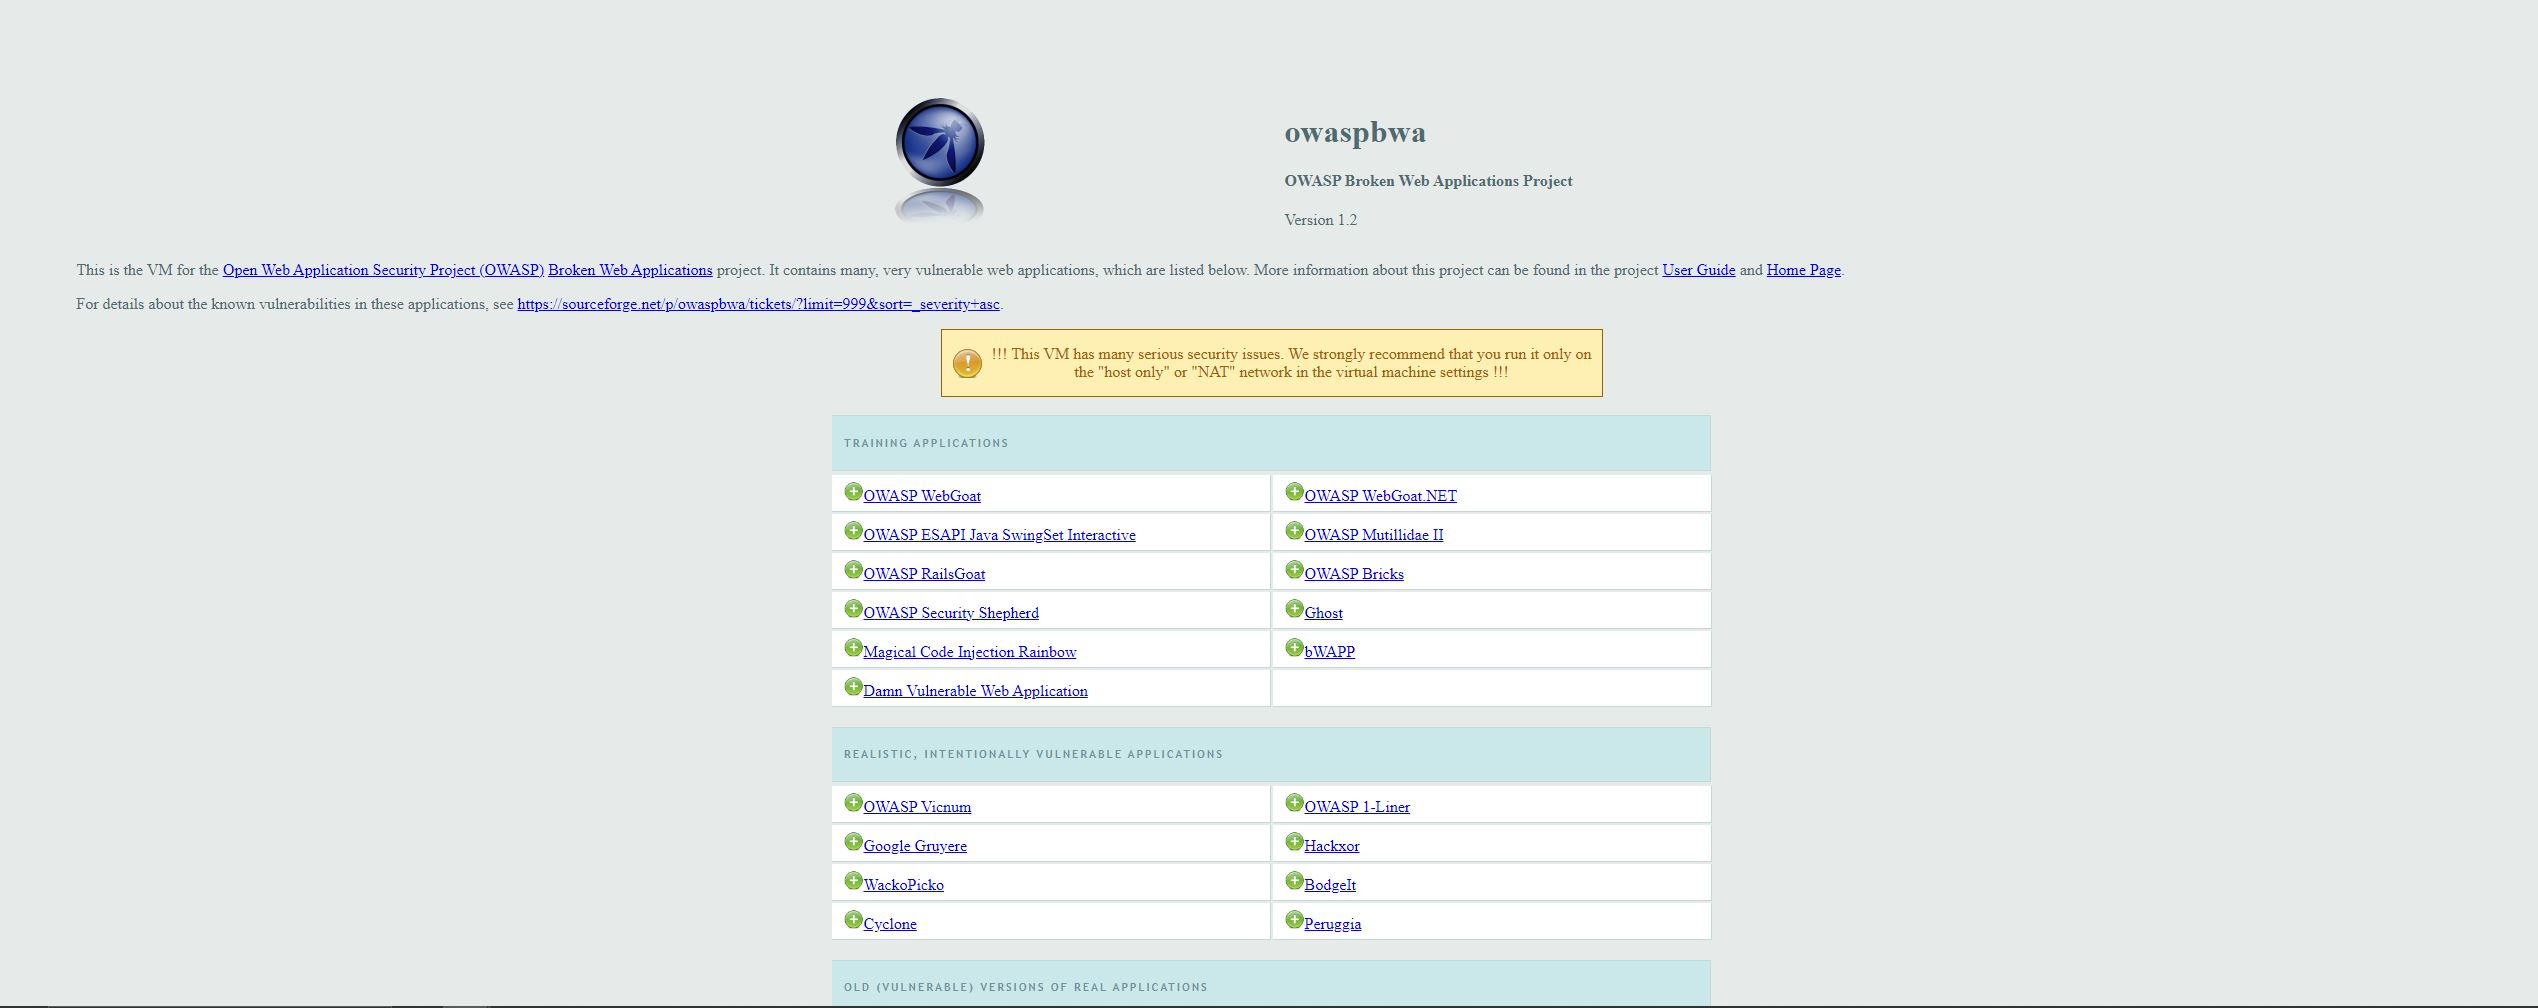
\includegraphics[width=15cm]{OWASPBWA.JPG}
     \caption{Captura de tela da OWASP BWA}
     \label{Label de referência para a imagem}
\end{figure}

\section{Mutillidae II}

A Mutillidae II é uma aplicação web open-source que oferece mais de 40 vulnerabilidades e desafios com vulnerabilidades encontradas desde a OWASP TOP Ten de 2007 até a de 2017. O ambiente conta com tutoriais e dicas para auxiliar no aprendizado e possui várias falhas simples de sempre exploradas para estimular o aprendizado da área \cite{url:owaspmuti}. Na Figura 2 é possível ver uma das páginas da Mutillidae II.

\begin{figure}[!htb]
     \centering
     \includegraphics[width=15cm]{Questão8.JPG}
     \caption{Captura de tela da Mutillidae II}
     \label{Label de referência para a imagem}
\end{figure}

%mutillidae 2
\chapter{Vulnerabilidades}

\section{Introdução}

A OWASP é uma organização sem fins lucrativos que por projetos open-source aspira auxiliar no desenvolvimento de aplicações e ambientes mais seguros. Dentre seus projetos existe a OWASP TOP:10 focado em informar aos profissionais de segurança e demais pessoas interessadas o estado atual da segurança mundial, quais tipos de vulnerabilidades tem sido mais exploradas e com isso chamar atenção para as falhas mais comumente exploradas por invasores, mostrando assim aspectos novos a serem observados com mais atenção nas aplicações. É importante frisar que vários tipos de vulnerabilidades são difíceis de serem quantificadas e monitoradas, por isso a OWASP não se baseia apenas em números de detecções, mas também no estado da arte, publicações e estudo de vulnerabilidades atuais \cite{url:OWASP}.

No ano de 2021 a OWASP TOP:10 publicou um novo informativo, classificando distintamente os tipos de vulnerabilidades antes previstos, criando categorias e alterando também o ranking de cada tópico. Neste ano os tópicos se baseiam muito na adequação as leis que envolvem a proteção de dados dos usuários. Na Figura 3 são apresentados os 10 maiores riscos do ano de 2021 segundo a OWASP.

\begin{figure}[!htb]
     \centering
     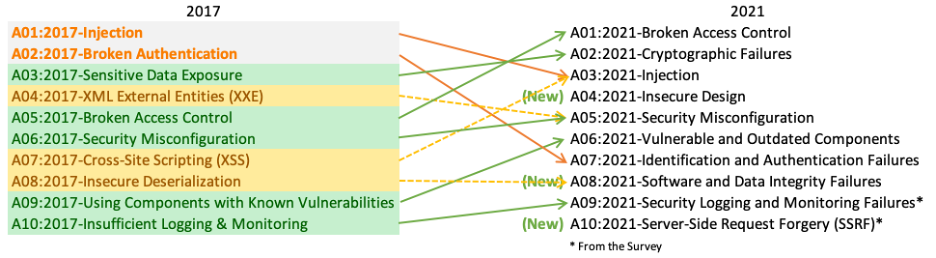
\includegraphics[width=15cm]{mapping.png}
     \caption{Top 10 Web Application Security Risks~\cite{url:OWASP}}
     \label{Label de referência para a imagem}
\end{figure}

% Vulnerabilidades 0day

\section{Broken Access Control}

Broken Access Control é um tipo de vulnerabilidade caracterizada pelo acesso a um ativo indevidamente por um usuário, sistema ou dispositivo não autorizado \cite{hassan2018quantitative}. Em sistemas as permissões de acesso deveriam ser bem definidas. Um sistema de hotelaria, por exemplo, não deveria permitir que um usuário autenticado como um comprador crie anúncios de quartos de Hotel através de um perfil administrativo. Na máquina Mutillidae II \cite{Jeremy2022} existe um exemplo de Broken Access Control, causada por cada usuário ter um \textit{uid} fixo e ordenado crescentemente. Para explorar a falha basta inserir credenciais válidas de qualquer usuário e alterar o \textit{uid} enviado na requisição em um valor de perfil com acessos administrativos.

\section{Cryptographic Failures}

Cryptographic Failures são as vulnerabilidades que expõem dados sensíveis de uma aplicação por conta de uma criptografia fraca ou inexistente \cite{nagoriquantum}. Os dados podem ir desde informações médicas até senhas ou números de cartão de crédito. Nas aplicações modernas os dados passam por manipulações de dados em repouso e em trânsito, tornando ainda mais necessário um controle rígido de criptografia para que essas vulnerabilidades sejam dificilmente aproveitadas. Este tipo de vulnerabilidade estava em terceiro lugar no ano de 2017, mas subiu para segundo lugar no ano de 2021 \cite{url:OWASP}, pois problemas de segurança causados por senhas \textit{hard-coded} tem se tornado muito comuns.

\section{Injection}

Injection é a classe de vulnerabilidades que engloba as falhas que ocorrem no momento que um dado é injetado em uma aplicação e consegue com isso alterar o comportamento planejado da aplicação, tornando, por exemplo, uma simples \textit{string} que serviriam como nome em um código malicioso executável \cite{9319139}. Essas falhas geralmente ocorrem por uma falta de validação das entradas ou uma neutralização imprópria das entradas das aplicações. Como exemplo de Injection temos um caso de SQL Injection, onde se a aplicação tiver dentro de seu código uma execução semelhante a "query = 'SELECT * FROM users WHERE id=' + getParamer("id") + ';'" seria possível dar como id o valor "' or 1=1'" e alterar o sentido original da query já que ela foi projetada para retornar os usuários onde o \textit{id} é igual ao informado, mas com esta injeção toda a tabela é retornada como resposta.

\section{Insecure Design}

Insecure Design é a classe de vulnerabilidades existentes quando um projeto possui problemas de segurança de forma que mesmo que as melhores práticas de desenvolvimento sejam utilizadas o sistema ainda continuará a ser inseguro. Então a causa da falha já faz parte do design escolhido para o projeto que podem levar a, por exemplo, vazamento de informações da aplicação \cite{9935837}. Uma das vulnerabilidades da classe é justamente a "CWE-209 Geração de mensagem de erro contendo informações confidenciais", mas erros como armazenamento desprotegido de credenciais ou violação de limite de confiança também vão ser vulnerabilidades desta classe.

\section{Security Misconfiguration}

Security Misconfiguration em resumo são as falhas de segurança motivadas por falta de configuração ou configuração padrão em aplicações e/ou serviços \cite{6045929}. Quando um banco de dados é configurado com valores padrão e executado em porta padrão, ele carrega inúmeros problemas e falhas de segurança. Falhas que podem ser facilmente encontradas por códigos maliciosas que procuram automaticamente serviços executando em determinadas portas. Nas Security Miscunfigurations também estão faltas por falta de configurações de header.

\section{Vulnerable and Outdated Components}

Vulnerable and Outdated Components é a classe que engloba as vulnerabilidades que envolvem as falhas por conta de componentes de software datados ou que possuem falhas conhecidas que são adicionados ao serviço em questão \cite{galvao2022analysis}. Durante o desenvolvimento de novos serviços é difícil criar tudo do zero, sendo comum, que sejam utilizados componentes prontos de terceiro, o problema é que quando um componente com falha é adicionado em uma aplicação, essa aplicação obviamente herda a vulnerabilidade que pode ou não ter algum peso no contexto da aplicação. 

\section{Identification and Authentication Failures}

Identification and Authentication Failures é a classe que aloca as falhas que envolvem controle de autenticação, como quebra em gerenciamento de sessão de usuários por má implementação do serviço \cite{authentication}. Essas falhas podem ter origens como: não tratamento para força bruta, permissão de senhas fracas, permissão de usuários default, processos ineficiente de recuperação de credenciais, e reutilização de identificadores de sessão. Muitas ferramentas são desenvolvidas para automatizar a exploração dessas vulnerabilidades, no caso de não tratamento de força bruta é possível explorar com ataques de dicionário.

\section{Software and Data Integrity Failures}

Software and Data Integrity Failures é a classe de vulnerabilidades que se aproveitam da falta de confirmação de integridade do software e de dados \cite{integrity}. Pode ocorrer, por exemplo, quando uma aplicação usa fontes externas não confiáveis, quando não existe um pipeline seguro no CI/CD, quando um invasor pode obter acesso a dados e/ou estruturas que possam ser vistas e alteradas. 

\section{Security Logging and Monitoring Failures}

O item Security Logging and Monitoring Failures da OWASP TOP Ten vai além de apenas classificar falhas, mas visa abordar os tópicos de resposta e monitoriamento dos ataques realizados em um ambiente \cite{logging}. Esta etapa se mistura com vários itens do OWASP TOP Ten, uma vez que para um correto monitoramento é necessário ter os logs armazenados seguramente, portanto um design correto para isso é necessário assim como confirmar a integralidade dos logs para se necessário usar os mesmos como provas. Dentro dessa classe de falhas é importante entender que além de logs insuficientes nas aplicações, logs com dados sensíveis também podem gerar problemas de segurança e logs com dados demais podem dificultar o monitoramento.

\section{Server-Side Request Forgery}

Server-Side Request Forgery como o nome diz, é uma vulnerabilidade causada pela falsificação de uma requisição do lado do servidor e ela acontece quando o servidor recupera o conteúdo de uma requisição, mas por não validar o URL acaba não garantindo que a requisição chegue ao destino esperado, esta falha tem um CWE mapeada que é a CWE-918 \cite{jabiyev2021preventing}. Esta vulnerabilidade consegue enviar as requisições a destinatários mesmo quando protegidos por firewall, VPN ou outro ACL.
\chapter{Tecnologias de Desenvolvimento}

\section{Docker}

O Docker é um sistema de virtualização que se baseia no empacotamento e uso de ambientes em \textit{containers}. O Docker diferente de outros sistemas de virtualização não necessita de Hardware virtualizado e nem necessariamente de uma instalação completa de um S.O. dentro do \textit{container} \cite{7742298}. Para seu funcionamento ele usa algumas \textit{features} do \textit{kernel} como o Cgroups e o namespaces, essas features são utilizadas para poder rodar os processos independentemente. Este modelo permite uma melhor organização da infraestrutura e, em simultâneo, mantém os ambiente seguros já que eles são separados. A Figura 4 compara a execução de imagens em um Linux Container e em Docker.

\begin{figure}[!htb]
     \centering
     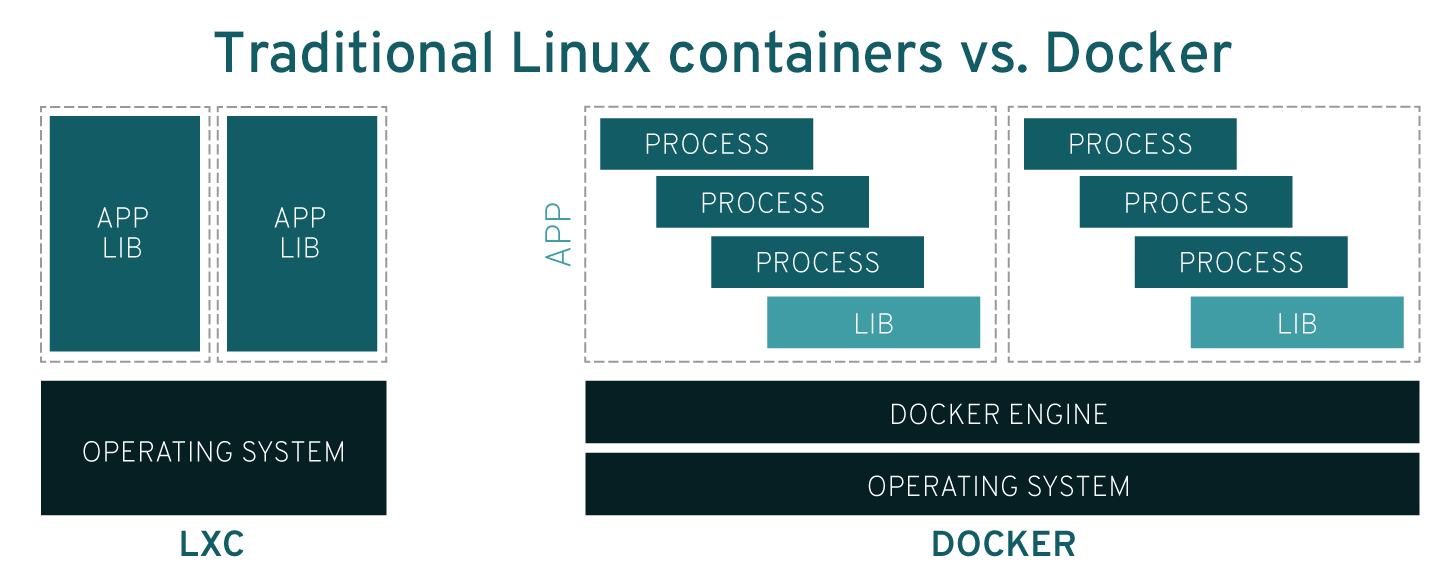
\includegraphics[width=15cm]{traditional-linux-containers-vs-docker_0.png}
     \caption{Figura do site RedHat sobre containers em Linux vs Docker~\cite{docker}}
     \label{Label de referência para a imagem}
\end{figure}

\section{Tecnologias de aplicação}

Além do Docker teremos algumas tecnologias que serão utilizadas no desenvolvimento do ambiente proposto.

\subsection{NodeJS}

Na aplicação de back-end a tecnologia de desenvolvimento será o NodeJS que é um \textit{runtime} de JavaScript que funciona em forma de execução assíncrona, permitindo a execução de código sem a necessidade de esperar o retorno de requisições \cite{7960064}. O Node foi criado pensando também em aplicações web escaláveis, sendo uma plataforma open-source multi-paradigmas.

\subsection{React}

O React é uma biblioteca do JavaScript que serve para a criação de interfaces de usuário. O React trabalha pensando em reaproveitamento de código criando componentes e pensando numa maior facilidade para descrição de estados e de conexão entre o CSS, JavaScript e HTML \cite{url:react}.

\subsection{SQLite}

O SQLite é um banco de dados relacional open-source prático e acessível que consegue atuar como o próprio servidor, já que ele insere seus dados dentro de si mesmo para funcionar. O nível de segurança desse banco não é tão alto, mas justamente isso também permite explorar outras vulnerabilidades dentro do ambiente \cite{5231398}.

\section{Ambiente local}

A imagem Docker estará disponível no repositório, após o download basta a execução que através do Dockerfile fará o ambiente ser configurado para permanecer sendo executado apenas de forma local, não permitindo que as aplicações sejam visualizadas pelo mundo exterior. Assim não haverá problemas com tráfego mal-intencionado na rede.
\chapter{Proposta de Desenvolvimento}

\section{Ambiente para Aprendizado e Prática de Técnicas de Segurança
Ofensiva em Aplicações Web Vulneráveis}

Existe uma similaridade entre a OWASP Broken, a Mutillidae e o ambiente proposto neste trabalho, os tipos de falhas encontrados nestas duas máquinas são muito semelhantes às falhas que serão desenvolvidas neste ambiente, porém a grande diferença é que este ambiente será desenvolvido em Docker com a intenção de facilitar a instalação e diminuir a ocupação de dados alocados em máquina.

O ambiente será desenvolvido com base em uma imagem Linux Ubuntu 22.04, para que possam ser exploradas não apenas falhas em aplicações web, mas falhas em aplicações web que levem a falhas em nível de sistemas operacional. Mesmo que isto custe um pouco mais de recursos em contra-ponto a uma aplicação que usaria \textit{docker-compose} para manter os serviços rodando separadamente.

As aplicações executadas dentro do Docker estarão por padrão disponíveis apenas ao Host de forma local para evitar que as vulnerabilidades sejam exploradas por atacantes.

\begin{figure}[!htb]
     \centering
     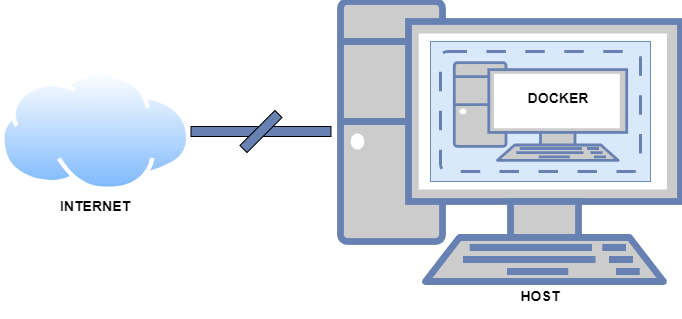
\includegraphics[width=15cm]{proposal.png}
     \caption{Ambiente proposto}
     \label{Label de referência para a imagem}
\end{figure}

A imagem docker do Ubuntu será alterada para conter alguns serviços, sendo os principais estes três: back-end sendo desenvolvido em NodeJS, front-end desenvolvido em JavaScript com React e um banco de dados com SQLite.
Alguns microsserviços também estarão disponíveis para explorar falhas pontuais e estão indicadas corretamente pelo front-end da aplicação.

\section{Vulnerabilidades selecionadas}

\subsection{CWE-23: Relative Path Traversal}

Ocorre quando existem entradas externas para a criação do \textit{path} de um determinado diretório, porém a entrada não é neutralizada e valores como "../" conseguem participar do path. Isso pode permitir por exemplo que diretórios indevidos sejam acessados como entradas do estilo "../../../../etc/passwd".

\subsection{CWE-319: Cleartext Transmission of Sensitive Information}

Ocasionada quando o sistema realiza a transmissão de dados sensíveis ou críticos em texto plano e permite que usuários não autorizados interceptem o dado.

\subsection{CWE-328: Use of Weak Hash}

Quando o algoritmo de Hash não tem como produto um resumo forte o suficiente, ele fica vulnerável a ataques que encontrem a valor original através de ataques de pré-imagem, 2ª pré-imagem ou ataques de aniversário.

\subsection{CWE-74: Improper Neutralization of Special Elements in Output Used by a Downstream Component}

Vulnerabilidade de injeção baseada na falta de neutralização de caracteres especiais nos valores de entrada que podem alterar a forma de interpretação e execução da aplicação.

\subsection{CWE-209: Generation of Error Message Containing Sensitive Information}

Um designe inseguro de aplicação que permite que o usuário veja informações sobre o ambiente, os usuários e dados relacionados através dos erros gerados na aplicação.

\subsection{CWE-613: Insufficient Session Expiration}

Falha na aplicação que permite acesso por sessões antigas ou apenas com o ID de acesso.

\subsection{CWE-565: Reliance on Cookies without Validation and Integrity Checking}

Acontece quando a aplicação depende dos dados nos Cookies para a realização de operações críticas, mas a aplicação não garante que os Cookies são do usuário da sessão.
\chapter{Considerações Finais}

O aprendizado da área de segurança computacional pode ser muito complicado, por isso ambientes para testes de vulnerabilidades são tão importantes. Com esses ambientes pode-se testar técnicas, correções, ferramentas, scripts, entre tantas outras coisas. Por este motivo este trabalho está sendo desenvolvido aspirando facilitar o percurso inicial na área. Além disso, ambientes em formato de imagem para Máquinas Virtuais já existem em certa quantidade, mas ambientes preparados para rodar em Docker e com isso economizar recursos são mais escassos.

Para este ambiente foram inicialmente escolhidas 7 vulnerabilidades que ainda podem ser encontradas com certa facilidade em sistemas web pelo mundo. Será necessário realizar testes para confirmar se o ambiente fica realmente segregado a fim de que máquinas usadas para testes não sejam vítimas de ataques enquanto usam o ambiente proposto.

\section{Cronograma}

\begin{center}
\begin{table}[!htb]
\begin{tabular}{|l|l|l|l|l|l|}
\hline
Etapa                                  & Março                  & Abril                  & Maio                   & Junho                  & Julho                  \\ \hline
Desenvolvimento do Back-end em NodeJS  & \multicolumn{1}{c|}{X} & \multicolumn{1}{c|}{X} &                        &                        &                        \\ \hline
Desenvolvilmento do Front-end em React & \multicolumn{1}{c|}{X} & \multicolumn{1}{c|}{X} &                        &                        &                        \\ \hline
Integração do Front-end com o Back-end &                        & \multicolumn{1}{c|}{X} & \multicolumn{1}{c|}{X} &                        &                        \\ \hline
Conclusão de escrita da monografia     &                        &                        & \multicolumn{1}{c|}{X} &                        &                        \\ \hline
Defesa de projeto                      &                        &                        &                        & \multicolumn{1}{c|}{X} &                        \\ \hline
Ajustes e envio final                  &                        &                        &                        &                        & \multicolumn{1}{c|}{X} \\ \hline
\end{tabular}
\end{table}
\end{center}

%%%%%%%%%%%%%%%%%%%%%%%%%%%%%%%%%%%%%%%%%%%%%%%%%%%%%%%%%%%%%%%%%%%%
%%% Elementos pós-textuais                                       %%%
%%%%%%%%%%%%%%%%%%%%%%%%%%%%%%%%%%%%%%%%%%%%%%%%%%%%%%%%%%%%%%%%%%%%

\postextual
% \bibliography{references}
\printbibliography[title={REFERÊNCIAS}]
\end{document}




% LocalWords:  pdf ufscthesisrn abntex PPGCC Zambonin pull request GitHub PRs
% LocalWords:  alexishuf Issues alpha dropin template cls shellescape ZIP Git
% LocalWords:  UNIXlike Makefile git submodule shame on you Overleaf english cd
% LocalWords:  overview PósGraduação Prof BU pdfpages bug BibTeX URLs at bst or
% LocalWords:  Available citealf url xurl brazil embeddedlogo autocontido pt
% LocalWords:  lmodern arial opensource Latin Modern nocapautoref ufscthesis
% LocalWords:  working directory pdflatex tex dijkstra diffie Saleem Ullman rdf
% LocalWords:  magic Distefano Abiteboul Forgy default Word captions userguide
% LocalWords:  noplainurl noabntexcite begin dedicatoria end doc abstracts EQM
% LocalWords:  corretude indentação oneside memoir feature SAD EQD bookmarks of
% LocalWords:  nopretextualbookmark listoffigures table contents logodir OUTDIR
% LocalWords:  jobname jobname-logo latexmkoutdir outdir latexmk filecontents
% LocalWords:  write thesis such main
